%%%%%%%%%%%%%%%%%%%%%%%%%%%%%%%%%%%%%%%%%%%%%%
% Modelo de Trabalho de Conclusão de Curso
% Engenharia Elétrica - CEFET - MG Nepomuceno
%
% Version 1.0 (16/02/2024)
%
% Author:
% Rosana Massahud (rosanamassahud@gmail.com)
%
% License:
% CC BY-NC-SA 3.0 (http://creativecommons.org/licenses/by-nc-sa/3.0/)
%
%%%%%%%%%%%%%%%%%%%%%%%%%%%%%%%%%%%%%%%%%%%%%%
\documentclass[12pt, A4, justify]{article}

\usepackage[brazil,brazilian]{babel}
\usepackage[utf8]{inputenc}
\usepackage[T1]{fontenc}
\usepackage{color}
\usepackage{amsmath, amsthm, amssymb, amsfonts}
\usepackage{bbding}
%\usepackage{Verbatim}
\usepackage{setspace}
\usepackage{subfigure}
\usepackage{multirow}
\usepackage{xcolor}
\usepackage[export]{adjustbox}

\usepackage{listings}% http://ctan.org/pkg/listings
\lstset{
  basicstyle=\ttfamily,
  mathescape
}
\pagenumbering{arabic}
%\renewcommand*{\thepage}{\small\arabic{page}}
\pagestyle{myheadings}
\usepackage{blindtext}
\makeatletter
\def\ps@myotherheadings{%
  \def\@evenfoot{\thepage\hfil}%  -> page number then fill
  \def\@oddfoot{\hfil\thepage} %  -> fill, then page number
  \def\@oddhead{{\slshape\rightmark}\hfil} % remove the page number
  \def\@evenhead{\hfil\slshape\leftmark}%
  \let\@mkboth\@gobbletwo
  \let\sectionmark\@gobble
  \let\subsectionmark\@gobble
}

\makeatother
\usepackage{caption}

\captionsetup[figure]{singlelinecheck=false,justification=justified,format= hang,font=normalsize}

%---------------------------------------------
% LISTA DE SCRIPTS (PROGRAMAS/SOURCE CODE)
%---------------------------------------------
\let\lstlistoflistingsorig\lstlistoflistings
\addto\captionsbrazilian{%
  \renewcommand*{\lstlistlistingname}{\centering \large LISTA DE PROGRAMAS}%
  \renewcommand*{\lstlistingname}{PROGRAMA}%  
}


%\renewcommand{\lstlistoflistings}{%
%  \cleardoublepage\phantomsection\addcontentsline{toc}{chapter}{\lstlistlistingname}% Add toc line
%    \lstlistoflistingsorig
%}

\definecolor{codegreen}{rgb}{0,0.6,0}
\definecolor{backcolour}{rgb}{0.95,0.95,0.92}

\lstset{
  numbers=left,
  stepnumber=1,
  numbersep=5pt,
  numberstyle=\normalsize\color{black},
  basicstyle=\ttfamily\normalsize,
  keywordstyle=\color{blue},
  commentstyle=\color{gray},
  stringstyle=\color{codegreen},
  %breakatwhitespace=false,
  %keepspaces=true,
  showstringspaces=false,
  frame=single,
  backgroundcolor=\color{white}%\color{backcolour}
  }

\DeclareCaptionFont{black}{ \color{black} }
\DeclareCaptionFormat{listing}{
  \colorbox[cmyk]{0.43, 0.35, 0.35,0.01 }{
    \parbox{\textwidth}{\hspace{15pt}\vspace{10pt}#1#2#3}
  }
}

%\captionsetup[lstlisting]{ format=listing, labelfont=black, textfont=black, singlelinecheck=true, margin=0pt, font={bf,normalsize} }


\usepackage{titlesec}

\titlespacing\section{0pt}{12pt plus 4pt minus 2pt}{0pt plus 2pt minus 2pt}
\titlespacing\subsection{0pt}{12pt plus 4pt minus 2pt}{0pt plus 2pt minus 2pt}
\titlespacing\subsubsection{0pt}{12pt plus 4pt minus 2pt}{0pt plus 2pt minus 2pt}

\usepackage{hyphenat}
% Set up the images/graphics package
\usepackage{graphicx}
\setkeys{Gin}{width=\linewidth,totalheight=\textheight,keepaspectratio}
\graphicspath{{graphics/}}
\usepackage[a4paper,top=3cm,botton=2cm,left=3cm,right=2cm,footskip=1.5cm]{geometry}
%\geometry{a4paper,tmargin=3cm,bmargin=2cm,lmargin=3cm,rmargin=2cm,headheight=1.5cm, includefoot}

%Recortar os espacos em branco em torno da figura
\usepackage{lineno}


%Identar o primeiro paragrafo de cada secao
\usepackage{indentfirst}
% Definindo tamanho da identação
\setlength{\parindent}{1.2cm}
\setlength{\paperwidth}{21.59cm}
\setlength{\paperheight}{27.94cm}

\usepackage{lipsum}

%%%%%%%%%%%%%%%%%%%%%%%%%%%%%%%%%%%%%%
% Fazer lista de símbolos
\usepackage{nomencl}
\makenomenclature

\usepackage{ragged2e}


%%%%%%%%%%%%%%%%%%%%%%%%%%%%%%%%%%%%%%%%%%%%%%%%%%%%
% Renomeando as palavras do pacote BABEL - BRAZILIAN
%%%%%%%%%%%%%%%%%%%%%%%%%%%%%%%%%%%%%%%%%%%%%%%%%%%%
\addto\captionsbrazilian{%
  \renewcommand{\contentsname}%
    {\centering \large SUMÁRIO} % Sumário para SUMÁRIO
  \renewcommand{\figurename}%
    {FIGURA} % Figura para FIGURA
  \renewcommand{\tablename}%
    {TABELA} % Tabela para TABELA
  \renewcommand{\listfigurename} %
    {\centering \large LISTA DE FIGURAS} %Lista de Figuras para LISTA DE FIGURAS
  \renewcommand{\listtablename} %
    {\centering \large LISTA DE TABELAS} %Lista de Tabelas para LISTA DE TABELAS
  \renewcommand{\nomname} %
    {\centering \textbf{\large{LISTA DE ABREVIATURAS E SIGLAS}}}%Lista de abreviaturas e siglas
}



%%%%%%%%%%%%%%%%%%%%%%%%%%%%%%%%%%%%%%
% Configurando o Sumario, Lista de Tabelas e Figuras
%%%%%%%%%%%%%%%%%%%%%%%%%%%%%%%%%%%%%%
\makeatletter

\renewcommand \thesection {\@arabic\c@section}

\renewcommand{\section}{\@startsection
{section}%                   % the name
{1}%                         % the level
{0mm}%                       % the indent
{-\baselineskip}%            % the before skip
{0.5\baselineskip}%          % the after skip
%{\noindent\centering\Large\textbf}} % the style
{\noindent\normalsize\textbf}} % the style
\renewcommand{\subsection}{\@startsection
{subsection}%                   % the name
{2}%                         % the level
{0mm}%                       % the indent
{-\baselineskip}%            % the before skip
{0.5\baselineskip}%          % the after skip
{\noindent\normalsize\textbf}} % the style

\renewcommand{\subsubsection}{\@startsection
{subsubsection}%                   % the name
{3}%                         % the level
{0mm}%                       % the indent
{-\baselineskip}%            % the before skip
{0.3\baselineskip}%          % the after skip
{\noindent\normalsize\textbf}} % the style

%criar a subsubsubsection
\setcounter{secnumdepth}{4}
\newcounter{subsubsubsection}[subsubsection]
\makeatletter
\def\subsubsubsectionmark#1{}
\def\thesubsubsubsection {\thesubsubsection.\arabic{subsubsubsection}}

\newcommand\subsubsubsection{\@startsection{subsubsubsection}{4}{\z@}%
                            {-3.25ex\@plus -1ex \@minus -.2ex}%
                            {1.5ex \@plus .2ex}%
                             {\normalfont\normalsize\bf}}
\def\@chapter[#1]#2{%
  \ifnum \c@secnumdepth >\m@ne
    \refstepcounter{chapter}
    \typeout{\@chapapp\arabic{chapter}}
    \addcontentsline{toc}{chapter}{\protect{\@chapapp\space\thechapter:\space}#1}
  \else
    \addcontentsline{toc}{\textbf{chapter}}{#1}
  \fi
  \@makechapterhead{#2}
  \@afterheading}

%%%%%%%%%%%%%%%%%%%%%%%%%%%%%%%%%%%%%%%%%%%%%%%%%%%%%%%%%%%%%%%%%%%%
%O que entra entre os {} é que fica em FIGURA {} BLA BLA BLA
\renewcommand*\captionlabeldelim{}%
%%%%%%%%%%%%%%%%%%%%%%%%%%%%%%%%%%%%%%%%%%%%%%%%%%%%%%%%%%%%%%%%%%%%

\def\l@section{\@dottedtocline{1}{0em}{2.6em}}
\def\l@subsection{\@dottedtocline{2}{0em}{2.7em}}
\def\l@subsubsection{\@dottedtocline{3}{0em}{2.9em}}
\def\l@subsubsubsection{\@dottedtocline{4}{0em}{3.1em}}

\def\singlespace{
\vskip\parskip
\vskip\baselineskip
\def\baselinestretch{1}
\ifx\@currsize\normalsize\@normalsize\else\@currsize\fi
\vskip-\parskip
\vskip-\baselineskip
}

\def\onehalfspacing{
\vskip\parskip
\vskip\baselineskip
\def\baselinestretch{1.5}
\ifx\@currsize\normalsize\@normalsize\else\@currsize\fi
\vskip-\parskip
\vskip-\baselineskip
}

%definir a profundidade do indice

\makeatletter
\let\@tableofcontents=\tableofcontents
\def\tableofcontents{\@tableofcontents\thispagestyle{empty}}

\makeatother
%%%%%%%%%%%%%%%%%%%%%%%%%%%%%%%%%%%%%%
% FIM - Configurando o Sumario, Lista de Tabelas e Figuras
%%%%%%%%%%%%%%%%%%%%%%%%%%%%%%%%%%%%%% % Aqui estão todas as bibliotecas e definições



\begin{document}

%\maketitle

%\section{Introduction}

\thispagestyle{empty}
\begin{titlepage}

\begin{center}

\includegraphics[width=3cm]{graphics/600px-Logo_CEFET-MG_corte.png}\\
\vspace{0.5cm}
{\normalsize \textbf{CENTRO FEDERAL DE EDUCAÇÃO TECNOLÓGICA DE MINAS GERAIS \\
CAMPUS NEPOMUCENO}}

\vspace{0.8cm}
{\large \textbf{João Eduardo Silva Mendonça; Lucas Victor de Moura Texeira; Romário de Oliveira Barbosa}}

\vspace{6cm}

{\large \textbf{ELECTRONIC HEALTH MONITOR: \\ \vspace{0.5 cm} Inovação eletrônica no monitoramento da saúde.}} \\
\vspace{0.5 cm}

\vspace{4 cm}


\vspace{3cm}
{\large \textbf{NEPOMUCENO}} \\
{\large \textbf{2024}}
\end{center}
\end{titlepage}

\newpage
\thispagestyle{empty}

\newpage\ \newpage               % capa (obrigatório)
\thispagestyle{empty}
%\begin{titlepage}

\begin{center}

{\large \textbf{João Eduardo Silva Mendonça; Lucas Victor de Moura Texeira; Romário de Oliveira Barbosa}}

\vspace{6cm}

{\large \textbf{ELECTRONIC HEALTH MONITOR: \\ \vspace{0.5 cm} Inovação eletrônica no monitoramento da saúde.}} \\
\vspace{0.7 cm}
\end{center}

\hspace{6.5cm}\begin{minipage}{8 cm}
     \nohyphens{Trabalho de Conclusão de Curso apresentado no curso de Graduação em Engenharia Elétrica do Centro Federal de Educação Tecnológica de Minas Gerais como requisito parcial para obtenção do título de Bacharel em Engenharia Elétrica.}

    \vspace{0.6 cm}

    Orientador: Alencar Franco de Souza \\
    Co-orientador: Rosana Áurea Tonetti Massahud
\end{minipage}
\vspace{3 cm}


\vspace{3cm}
\begin{center}
{\large \textbf{NEPOMUCENO}} \\
{\large \textbf{2024}}
\end{center}
%\end{titlepage}              % folha de rosto (obrigatório)
\newpage \normalsize
%\thispagestyle{plain} comentei(rosana)
\thispagestyle{empty}

\vspace*{6cm}
\begin{center}



\vspace{1 in}
\begin{spacing}{1.0}
\begin{tabular}{|clc|} \hline

  \hspace{0.5cm} & & \\
  & Campos, Máira Rolla & \\
  C198d & \hspace{0.15in} Detecção de danos em vigas de aço por meio da análise do espectro de & \\
  & frequências / Maíra Rolla Campos. \- 2020. & \\
  & \hspace{0.15in} 65 f. : il., gráfs, tabs, fotos & \\
  & & \\ 
  & \hspace{0.15in} Dissertação apresentada ao Programa de Pós-Graduação em Engenharia & \\
  & de Civil & \\
  & \hspace{0.15in} Orientador: Cláudio José martins. & \\
  & \hspace{0.15in} Bibliografia: f. 59-62. & \\
  & \hspace{0.15in} Dissertação (mestrado) \- Centro federal de Educação Tecnológica de &\\
  & Minas Gerais, Departamento de Engenharia Civil. & \\
  & & \\
  & \hspace{0.15in} 1. Aço \- Estrutura \- Teses. 2. Análise modal \- Teses. 3. Pesquisa & \\
  & operacional \- Teses. 4. Falhas estruturais \- Teses. 5. Monitoramento de & \\
  & integridade estrutural \- Teses. 6. Efeiros de vibração \- Teses. I. Martins, & \\
  & Cláudio José. II. Centro Federal de Educação Tecnológica de Minas Gerais. & \\
  & departamento de Engenharia Civil. III. Título. & \\
  & & \\ 
  & CDD 624.182 & \\
  & & \\ \hline
\end{tabular}
\end{spacing}
\end{center}
\vspace{-0.4 cm}

\noindent Elaboração da ficha catalográfica pela bibliotecária Jane Marangon Duarte, CRB 6\textordmasculine 1592/ Cefet/MG

%\end{tabular}




 % ficha-catalográfica  (obrigatório)
% \thispagestyle{empty}
\begin{center} \textbf{ERRATA} \end{center}

\vspace{1 cm}

\hspace{0.5 cm} FERRIGNO, C. R. A. \textbf{Tratamento de neoplasias ósseas apendiculares com
    reimplantação de enxerto ósseo autólogo autoclavado associado ao plasma
    rico em plaquetas}: estudo crítico na cirurgia de preservação de membro em
cães. 2011. 128 f. Tese (Livre-Docência) - Faculdade de Medicina Veterinária e
Zootecnia, Universidade de São Paulo, São Paulo, 2011.

\begin{table}[htb]
    \center
    \footnotesize
    \begin{tabular}{|p{1.4cm}|p{1cm}|p{3cm}|p{3cm}|}
        \hline
        \textbf{Folha} & \textbf{Linha} & \textbf{Onde se lê} & \textbf{Leia-se} \\
        \hline
        1              & 10             & auto-conclavo       & autoconclavo     \\
        \hline
    \end{tabular}
\end{table}             % errata (opcional)
\thispagestyle{empty}
\begin{titlepage}

\begin{center}

{\large \textbf{NOME DO AUTOR}}

\vspace{5cm}

{\large \textbf{TÍTULO DO TRABALHO: \\ \vspace{0.5 cm} subtítulo do trabalho (se houver)}} \\
\vspace{0.7 cm}
\end{center}

\hspace{6.5cm}\begin{minipage}{8 cm}
     \nohyphens{Trabalho de Conclusão de Curso apresentado no curso de Graduação em Engenharia Elétrica do Centro Federal de Educação Tecnológica de Minas Gerais como requisito parcial para obtenção do título de Bacharel em Engenharia Elétrica.}


\end{minipage}

\vspace{1 cm}

Aprovado em 18 de dezembro de 2023.
\vspace{2 cm}

\begin{center}
\rule{10 cm}{1pt} \\
\vspace{0.3 cm}

Título Nome \\

\vspace{0.2 cm}

Instituição

\vspace{1 cm}

\rule{10 cm}{1pt} \\
\vspace{0.3 cm}

Título Nome \\

\vspace{0.2 cm}

Instituição

\vspace{1 cm}

\rule{10 cm}{1pt} \\
\vspace{0.3 cm}

Título Nome \\

\vspace{0.2 cm}

Instituição

\end{center}
\end{titlepage}          % folha de aprovação (obrigatório)
\thispagestyle{empty}
\vspace*{18cm}

\begin{flushright}
  {\textit{Ao familiares e amigos,          \\ 
  pelo apoio em nossa graduação. \\
  \vspace{0.2 cm}
  DEDICO
  }}
\end{flushright} \normalsize        % dedicatória (opcional)
% \thispagestyle{empty}

\begin{center}
{\large \textbf{AGRADECIMENTOS}}
\end{center}



\begin{trivlist}  \itemsep 2ex  \normalsize

\item \lipsum[2]

\lipsum[1-3]

\end{trivlist}     %agradecimentos (opcional)
% 
% ********** Epígrafe

%% não numerar a página
\thispagestyle{empty}

\vspace*{10 cm}
 
\begin{flushright}
\begin{minipage}[t]{6.8cm} {
\vspace{7cm}
\nohyphens{\small{\sl{
tempo de rasgar e tempo de remendar;\\
tempo de ficar calado e tempo de falar.\\
Há tempo de amar e tempo de odiar;\\
tempo de guerra e tempo de paz.}}}
\begin{flushright}
\it{Eclesiastes 3, 7-8}
\end{flushright}
}
\end{minipage}
\end{flushright}           %epigrafe (opcional)
% \newpage
\thispagestyle{empty}
\vspace{1.5cm}
\begin{center}
{\large{\textbf{RESUMO}}}
\end{center}
\vspace{0.5cm}

\begin{spacing}{1.0}
\noindent A dengue é a doença viral transmitida por um arbovírus que mais rapidamente se espalha no mundo. Seu principal vetor é o mosquito \emph{Aedes aegypti}, muito adaptado ao meio urbano. No caso do Brasil, já podemos observar o grande surto epidêmico em 2011, principalmente depois da entrada do sorotipo 4 no país. A incidência de dengue mostra uma clara dependência das variações sazonais. Além disso, fatores relacionados a cada indivíduo envolvido no processo podem ser analisados dentro do contexto epidêmico. Os modelos matemáticos têm sido cada vez mais utilizados para se tentar mapear os comportamentos das doenças infecciosas. Adicionado a eles, utiliza-se também de recursos computacionais para simulações agregando características comportamentais dos indivíduos e outros aspectos relevantes ao estudo. Para estudar a propagação da doença propomos um modelo matemático e computacional a partir de autômatos celulares, o qual procura identificar os fatores que contribuem para a proliferação da dengue. O foco principal do trabalho é a interação entre os indivíduos envolvidos no processo de espalhamento da dengue, levando em conta aspectos espaciais. Por meio da teoria de modelos baseados em indivíduos e com recursos computacionais, construimos um autômato celular, considerando as características comportamentais das epidemias de dengue - implementando o comportamento cíclico da doença, e as interações indivíduo a indivíduo numa região hipotética. O modelo nos permitiu capturar informações gerais sobre a dengue além de comportamentos essenciais dos indivíduos, afirmando a característica básica desse tipo de modelagem: a partir de regras simples, capturar informações complexas embutidas nas interações entre os agentes. Os resultados obtidos nos conferiram a importância das interações entre o vetor e o hospedeiro na permanência da doença. Apesar de tratarmos uma região hipotética obtivemos comportamentos semelhantes aos encontrados na natureza. As principais particularidades encontradas nos remetem às interações, densidades populacionais e, fundamentalmente, aos deslocamentos dos indivíduos e às elevadas taxas de casos assintomáticos da doença.
\end{spacing}

\vspace{1.5ex}

\noindent {\bf Palavras-chave}: Epidemias. Dengue. Modelos baseados em indivíduos. Autômatos celulares.

             % resumo (obrigatório)
% \newpage
\thispagestyle{empty}
\vspace{1.5cm}
\begin{center}
{\large{\textbf{ABSTRACT}}}
\end{center}
\vspace{0.5cm}
 \hyphenation{especially automata taking epidemics capture behaviors}
\begin{spacing}{1.0}
\noindent Dengue is a viral disease transmitted by an arbovirus that quickly spreads around the world. Its main vector is the mosquito \emph{Aedes aegypti} urban environment well adapted. In Brazil, it is already observed a large outbreak in 2011 especially after serotype 4 arrived in the country. Dengue's incidence shows a clear dependence on seasonal variations. In addition, factors related to each individual involved in the process can be analyzed within epidemic context. Mathematical models have been increasingly used to try to map infectious diseases behavior. Added to them, it is also used computing resources for simulations by aggregating individual behavioral characteristics and other research relevant aspects. To study disease spread, we propose a mathematical and computer model from cellular automata, which seeks to identify factors that contribute to dengue spread. The main focus of this paper is the interaction among spread dengue involved individuals taking into account spatial aspects. Through individual based modelling theory and with computational resources, build cellular automata, considering dengue epidemics behavioral characteristics - implementing the cyclical disease behavior and individual to individual interactions in a hypothetical region. The model allowed us to capture dengue general information as well as individuals' essential behaviors, claiming this type of modeling basic characteristic: from simple rules, capture complex information embedded in agents interactions. The results gave us the importance vector and host interactions to disease maintenance. Despite treating a hypothetical region the obtained behaviors were similar to those found in nature. The main found peculiarities are related to interactions, population densities and, crucially, to individuals movements and the high rates of disease asymptomatic cases.

\end{spacing}

\vspace{1.5ex}

\noindent {\bf Keywords}: Epidemics. Dengue. Individual-Based Modelling. Cellular automata.


           % resumo em lingua estrangeira (obrigatório)
\thispagestyle{empty}

% \newpage
% \pagestyle{empty}
% \listoffigures

% \newpage
% \thispagestyle{empty}
% \listoftables

% \newpage
% \thispagestyle{empty}
% \lstlistoflistings

% %lista de símbolos
% \newpage
% \thispagestyle{empty}
% \lstlistoflistings

%lista de símbolos
%\newpage
%\thispagestyle{empty}

% \newpage
% \thispagestyle{empty}
% 
\vspace{2 cm}

\nomenclature{AHSS}{Aços Avançados de Alta Resistência (\textit{Advanced Sigh Strength Steel})}
\nomenclature{ALT}{Alongamento Total}
\nomenclature{ASTM}{\textit{American Society for Testing and Materials}}
\nomenclature{BC}{Aço com Baixo Teor de Carbono}
\nomenclature{BH}{Aço Endurecível pela Cura da Pintura (\textit{Bake Hardening})}
\nomenclature{CP}{Aço Multifásico (\textit{Complex Phase})}
\nomenclature{DP}{Aço Bifásico (\textit{Dual Phase Steel})}
\nomenclature{EBSD}{Difração de Elétrons retroespalhados (\textit{Eletron Backscatter Diffraction})}
\nomenclature{HPF}{Aços Estampados a Quente (\textit{Hot Press Forming})}
\printnomenclature

\newpage
\thispagestyle{empty}
%\nomname
\centering \textbf{\large{LISTA DE ABREVIATURAS E SÍMBOLOS} }

\vspace{2 cm}
\justifying
\begin{tabular}{l l}
    bpm & Batimentos por minuto\\[10pt]
    Sp02 & Saturação de oxigênio medida pelo oxímetro de pulso\\[10pt]
    OMS & Organização Mundial da Saúde\\[10pt]
    DCV & Doenças Cardiovasculares\\[10pt]
    Fc & Frequência Cardíaca\\[10pt]
    Tc & Temperatura corporal\\[10pt]
    PWM & Pulse Width Modulation\\[10pt]
    EEPROM & Electrically Erasable Programmable Read-Only Memory\\[10pt]
    SRAM & Static Random-Access Memory\\[10pt]
    USB & Universal Serial Bus\\[10pt]
    GPIO & General-Purpose Input/Output\\[10pt]
    UART & Universal Asynchronous Receiver-Transmitter\\[10pt]
    I2C & Inter-Integrated Circuit\\[10pt]
    IPS & Inter-Peripheral System\\[10pt]
    SPI & Serial Peripheral Interface\\[10pt]
    COPI & Controller Out, Peripheral In\\[10pt]
    CIPO & Controller In, Peripheral Out\\[10pt]
    SCK & Serial Clock\\[10pt]
    SCL & Serial Clock Line\\[10pt]
    SDA & Serial Data Line\\[10pt]
    CS & Chip Select\\[10pt]
    Wi-Fi & Wireless Fidelity\\[10pt]
    ROM & Read-Only Memory\\[10pt]
\end{tabular}

\newpage
\thispagestyle{empty}
\begin{tabular}{l l}
    MHz & Megahertz\\[10pt]
    E/S & Entradas e Saídas\\[10pt]
    JS & Javascript\\[10pt]
    RN & React-Native\\[10pt]
\end{tabular}
           
%\listofequations

\newpage
\thispagestyle{empty}
\textbf{\onehalfspacing
\tableofcontents
}
\newpage

           % listas e sumário (obrigatório)
\pagestyle{myheadings}
\setcounter{page}{16} % ajustar essa numeração, contando as páginas pré textuais, a partir da folha de rosto.

\justifying

\section{INTRODUÇÃO}

\lipsum[1-6]

\subsection{Objetivos}

\lipsum[1-1]

            % introdução (obrigatório)
\section{REFERENCIAL TEÓRICO}

O texto a seguir constitui todo o embasamento teórico para a realização deste trabalho de conclusão de curso, que tem como objetivo desenvolver um dispositivo eletrônico acessível para monitorar a frequência cardíaca, saturação de oxigênio e temperatura corporal.

\subsection{Frequência cardíaca (Fc)}

As doenças cardiovasculares (DCV) são as principais causas de mortes no mundo, sendo um grave problema de saúde pública (Mendonça 2016). Segundo a Organização Mundial de Saúde (OMS), cerca de 17,9 milhões de pessoas perderam a vida devido a complicações cardiovasculares em 2019, representando aproximadamente 32\% das mortes globais.
Frequência cardíaca ou ritmo cardíaco é o número de vezes que o coração bate por minuto (bpm). Esse batimento pode ser dividido em várias fases – ciclo cardíaco (Ferreira, Almeida et al. 2007). Os batimentos cardíacos normais variam conforme a idade e o estado de saúde da pessoa, as tabelas a seguir mostram os parâmetros:

\subsection{Saturação (Sp02)}

\subsection{Temperatura corporal (Tc)}

\subsection{Arduino}

\subsubsection{Tipos de Arduino}

\subsubsubsection{Arduino UNO}

\subsubsubsection{Arduino Nano}

\subsubsubsection{Arduino Mega}

\subsection{Sensor MAX30102}

\subsection{Sensor MLX90614}

\subsection{Display Oled}

\subsection{Modulo GSM SIM800L}     % referencial teórico (obrigatório)
% \section{METODOLOGIA}

\lipsum[1-2]

\subsection{Seção}

\lipsum[1-2]           % material e mátodos (metodologia) (Obrigatório)
% \section{RESULTADOS E DISCUSSÕES}
\section{RESULTADOS ESPERADOS}

Espera-se que o dispositivo seja capaz de ler com precisão, eficiência e efiácia os sinais vitais. Com relação ao aplicativo, espera-se q a interface seja de fácil utilização e contemple todos os dados medidos, através de tabelas e/ou gráficos.
% \subsection{Exemplos de gráficos e figuras}

% Para inserir figuras no \LaTeX é utilizado o comando \textsc{includegraphics}. Para indexar essa figura precisamos do ambiente \textsc{figure}. Veja como exemplo a Figura \ref{fig:figura1}. Neste template, as figuras devem ser armazenadas fisicamente no diretório \textsc{graphics}.
% Ajuste a label e a legenda adequadamente.

% \begin{figure}   %\captionsetup{singlelinecheck=false,justification=justified,format= hang,font=normalsize}
%     \caption{Exemplo de figura.}
%     \vspace{-0.5 cm}
%     \begin{center}
%     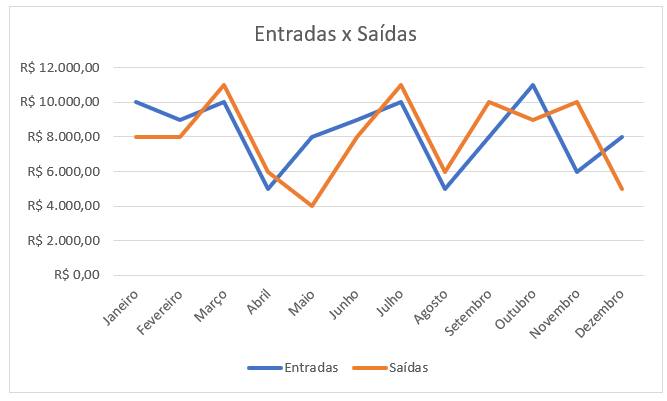
\includegraphics[scale=0.8]{graphics/exemploFigura1.png}
%     \end{center}
%     \vspace{-0.3 cm}
%     \small{Fonte: EXCELEASY (2024).}
%     \label{fig:figura1}
% \end{figure}

% \subsection{Exemplo de tabelas}

% Pra Quadros ou Tabelas, recomenda-se  a ajuda do site ``Tables Generator'' (TABLES GENERATOR, 2024). Além disso, para indexação é necessário o ambiente \texttt{table}. Veja um exemplo na Tabela

% \begin{table}[h]
% \centering
% \caption{Exemplo de tabela.}
% \begin{tabular}{|l|l|l|l|}
% \hline
% & \textbf{A} & \textbf{B} & \textbf{C} \\
% \hline
% 1 & 11         & 12         & 13         \\
% 2 & 0          & 2          & 3          \\
% 3 & 25         & 26         & 27    \\     
% \hline    
% \end{tabular}
% \vspace{0.2 cm}

% \small{Fonte: A autora.}
% \end{table}

% \normalsize



% \subsection{Exemplo de Programas, Scripts ou Algoritmos}

% Programas ou Scripts podem ser escritos em \LaTeX usando o pacote \texttt{lstlisting}. É importante que esse pacote seja configurado adequadamente de acordo com a linguagem de programação utilizada. Como exemplo, veja o Programa que está escrito em Python. Neste template, a configuração do pacote está discponível no arquivo \texttt{estrutura.tex}.

% \begin{lstlisting}[caption={Função Eliminação de Gauss},label={prog:gauss},language=Python]
% import numpy as np

% def gauss(n, A, b):#algoritmo do livro do Ruggiero
%     '''
%     supor que o elemento que estah na posicao akk 
%     eh diferente de zero no inicio da etapa k
%     '''
%     A_copy = A.copy()
%     b_copy = b.copy()
%     for k in range(0,n-1):
%         for i in range(k+1,n):
%             m = float(A_copy[i][k]/A_copy[k][k])
%             for j in range(k,n):
%                 A_copy[i][j] = float(A_copy[i][j]-
%                     float(m*A_copy[k][j]))
%             b_copy[i] = float(b_copy[i]) - float(m*b_copy[k])
%             A_copy[i][k] = 0
%     #fase da resolucao
%     return retroativa(n,A_copy,b_copy)
% \end{lstlisting}
% \small{Fonte: A autora}

% \normalsize


%  \lipsum[1-2]



            % resultados e discussões (obrigatório)
% \section{CONCLUSÃO}

\lipsum[1-3]             % conclusão ou considerações finais (obrigatório)
\addcontentsline{toc}{section}{\protect\numberline{}REFERÊNCIAS}
\section*{REFERÊNCIAS BIBLIOGRÁFICAS}

% Para escrever corretamente as referências bibliográficas e citações, recomendamos o site
% https://more.ufsc.br/

\\

\singlespacing 
\noindent EXCELEASY. Gráfico de linhas no Excel. Disponível em: https://exceleasy.com.br/grafico-de-linhas-no-excel/grafico-de-linhas-no-excel/ Acesso em: fev. 2024.

\\

\singlespacing
\noindent TABLES GENERATOR. Disponível em: https://www.tablesgenerator.com/ Acesso em: fev. 2024.
\\
% No manual de normalização de trabalhos acadêmicos do CEFET, temos a seguinte lista de Referências usadas como exemplo

\noindent BRASIL. Congresso Nacional. Lei nº 14.040, de 18 de agosto de 2020. Estabelece normas educacionais excepcionais a serem adotadas durante o estado de calamidade pública reconhecido pelo Decreto Legislativo nº 6, de 20 de março de 2020; e altera a Lei nº 11.947, de 16 de junho de 2009. Diário Oficial da União. Poder Legislativo, Brasília, 19 ago. 2020. Edição: 159, Seção 1, p. 4. Disponível em: https://www.in.gov. br/en/web/dou/-/lei-n-14.040-de-18-de-agosto-de-2020-272981525. Acesso em: 16 mar. 2021.

\singlespacing{
\noindent CHAUÍ, Marilena de Souza. \textbf{Convite à filosofia.} 13. ed. São Paulo: Ática, 2009. 424 p. }
\\

\singlespacing
\noindent DEMO, Pedro. \textbf{Conhecimento moderno}: sobre ética e intervenção do conhecimento. 3. ed. Petrópolis: Vozes, 1999, 317 p. 
\\

\singlespacing
\noindent \rule{2cm}{0.10mm}\textbf{ Metodologia do conhecimento científico.} São Paulo: Atlas, 2000, 216 p.
\\

\singlespacing
\noindent \rule{2cm}{0.10mm} \textbf{A educação do futuro e o futuro da educação}. Campinas, SP: Autores Associados, 2005, 191 p. (Coleção educação contemporânea). 
\\

\singlespacing
\noindent ELIAS, Norbert. A sociedade dos indivíduos. Rio de Janeiro: Jorge Zahar, 1994. 201 p. 
\\

\singlespacing
\noindent GEERTZ, Clifford. \textbf{A interpretação das culturas}. 13. reimpr. Rio de janeiro: LTC, 1989. 213 p. 
\\

\singlespacing
\noindent GIL, Antônio Carlos. \textbf{Como elaborar projetos de pesquisa}. 5. ed. São Paulo: Atlas, 2010. xiv, 184 p. 
\\

\singlespacing
\noindent LARAIA, Roque de Barros. \textbf{Cultura}: um conceito antropológico, 14. ed. Rio de Janeiro: Zahar, 2001. 
\\

\singlespacing
\noindent LATOUR, Bruno. \textbf{Ciência em ação}: como seguir cientistas e engenheiros sociedade afora. Tradução de Ivone C. Benedetti. 2. ed. São Paulo: Ed. UNESP, 2011. 422 p. 
\\

\singlespacing
\noindent MARCONI, Marina de Andrade; LAKATOS, Eva Maria. \textbf{Fundamentos de metodologia científica}. 7. ed. São Paulo: Atlas, 2010. xvi, 297 p. 
\\

\singlespacing
\noindent MEDEIROS, João Bosco. \textbf{Redação científica}: a prática de fichamentos, resumos, resenhas. 12. ed. São Paulo: Atlas, 2014. 331 p. 
\\

\singlespacing
\noindent PINTO, Álvaro Vieira. \textbf{O conceito de tecnologia}. Rio de Janeiro: Contraponto, 2005. xiv, 531 p. v. 1. 
\\

\singlespacing
\noindent PINTO, Álvaro Vieira. \textbf{O conceito de tecnologia}. Rio de Janeiro: Contraponto, 2005. xii, 794 p. v. 2 
\\

\singlespacing
\noindent SPALDING, M.; RAUEN, C.; VASCONCELLOS, L. M. R. de; VEGIAN, M. R. da C.; MIRANDA, K. C.; BRESSANE, A.; SALGADO, M. A. C. Desafios e possibilidades para o ensino superior: uma experiência brasileira em tempos de COVID-19. \textbf{Research, Society and Development}, [S. l.], v. 9, n. 8, 2020.Disponível em: https://rsdjournal. org/index.php/rsd/article/view/5970. Acesso em 29 mar. 2021.           % referências bibliográficas (obrigatório)

% \addcontentsline{toc}{section}{\protect\numberline{}GLOSSÁRIO}
% %%
%% Capítulo : GLOSSÁRIO
%%
\section*{\centering GLOSSÁRIO}

%\begin{center}
%    \large \textbf{ANEXO A - GLOSSÁRIO}
%\end{center}


Glossário de termos epidemiológicos apresentados no texto desta dissertação.

\begin{description}
\item[Anautógeno, mosquito:] É a espécie de mosquitos onde as fêmeas necessitam de alimentação sanguínea para adquirirem os aminoácidos necessários à produção dos ovos. Machos e fêmeas podem ainda alimentar-se de glicídios obtidos do néctar de flores e de suco de frutos e utilizá-los como combustível energético para o vôo e outras atividades.
\item[Anticorpo:] Proteína produzida no sangue de vertebrados após exposição a um antígeno. O anticorpo liga-se especificamente ao antígeno e assim estimula sua inativação por outros componentes do sistema imune. A maior classe de anticorpos são imunoglobulinas A ou IgA, encontrada predominantemente em secreções corporais tais como saliva. As IgM e IgG são tipicamente produzidas sequencialmente em resposta a infecções por microparasitas; IgE é frequentemente elevada na resposta a infecção helmíntica. Somente IgG é capaz de cruzar a placenta para conferir imunidade materna.
\item[Antígeno:] Proteína estranha ao organismo que elicita em resposta imune específicamente dirigida contra ela.

\item[Arbovírus:] Vírus que usam artrópodes como vetores a são transmitidos através da saliva destes para o hospedeiro definitivo. Ex.: dengue e febre amarela.

\item[Arbovirose:] v. arbovírus.

\item[Artrópode:] São animais invertebrados caracterizados por possuírem membros rígidos e articulados e terem vários pares de pernas. Compõem o maior filo de animais existentes, representados pelos gafanhotos (insetos), aranhas (aracnídea), caranguejos (crustáceos), centopeias (quilópodes) e embuás (diplópodes).

\item[Ciclo gonotrófico:] Ciclo vital do mosquito (ciclo completo de desenvolvimento ovárico do mosquito), ou seja, o tempo que decorre entre a ingestão de sangue (através da picada) e a postura dos ovos.

\item[Contato, taxa:] Taxa de contato entre susceptíveis e infectados. Medido em indivíduos por unidade de tempo.

\item[Endemia:] Termo usado para descrever níveis de infecção que não exibem grande flutuação temporal em um determinado lugar. Para microparasitas tais como sarampo, o termo é usado para indicar uma infecção que persiste em uma população por longo tempo sem necessidade de ser reintroduzida por uma fonte externa. Endemicidade estável é o termo utilizado para uma doença transmissível que não mostra tendência secular para aumentar ou diminuir.

\item[Epidemia:] Rápido aumento nos níveis de uma infecção, típico dos microparasitas (com imunidade de longa duração e curtos tempo de geração). Uma epidmia é anunciada por um aumento exponencial no número de casos no tempo e um subseqüente declínio devido ao esgotamento do número de susceptíveis. Uma epidemia pode se originar pela introdução de um novo patógeno (ou linhagem) numa população anteriormente não exposta ao mesmo, ou pelo mesmo patógeno como resultado do aumento no número de susceptíveis algum tempo após uma epidemia prévia.

\item[Expectativa de vida:] O mesmo que longevidade, o tempo médio de vida dos indivíduos em uma população.

\item[Força de infecção:] Taxa per capita de infecção de susceptíveis.

\item[Holometábolo:] Holometábolo é um animal que tem metamorfose completa durante o seu desenvolvimento.
Nos insetos holometábolos o desenvolvimento é tido da seguinte forma: ovo, larva, pupa jovem, pupa adiantada, imago.

\item[Horizontal, transmissão:] Transmissão ocorrendo dentro de uma população entre seus indivíduos, mas que não inclui transmissão vertical.

\item[Imunidade:] 1) Estado em que um hospedeiro não é susceptível à uma infecção ou doença; ou 2) o mecanismo pelo qual isto é alcançado. O indivíduo adquire imunidade através de uma das três rotas: imunidade natural ou inata, geneticamente herdada ou adquirida através de anticorpos maternos; imunidade adquirida, conferida após contato com a doença; e imunidade artificial, após vacinação bem sucedida (também imunidade específica ou resistência). A imunidade específica é dividida em imunidade celular, atuando via células T e imunidade humoral envolvendo anticorpos e células B.

\item[Incidência:] Taxa de aparecimento de casos novos numa população. Classicamente medida como "taxa de ataque".

\item[Infecção:] Replicação de um microparasita em seu hospedeiro, podendo haver ou não doença.

\item[Infeccioso, período:] Período de tempo durante o qual infectados são capazes de transmitir a infecção para qualquer hospederio susceptível ou vetor com os quais entre em contato. Note que o período infeccioso pode não ser necessariamente associado com sintomas da doença.

\item[Infectado:] Hospedeiro que tem uma infecção.

\item[Intermediário, hospedeiro:] V. vetor.

\item[Latente, período:] Período da infecção em que o indivíduo é infeccioso para os susceptíveis. Em helmintos, é chamado de período pré-patente. Não confundir com período de incubação.

\item[Limiar de transmissão:]  Ocorre quando a taxa reprodutiva básica R0 de um parasita é igual 1. Abaixo deste limiar a doença é incapaz de se manter na população. Para parasitas de transmissão direta há um limiar de transmissão para o tamanho da população hospedeira.

\item[Mortalidade, taxa:] Mortes per capita numa população. A taxa de mortalidade é a recíproca da expectativa de vida de uma população.

\item[Oligossintomático:] que apresenta pouco ou quase nenhum sintoma da doença.

\item[Ovariolar:] Relativo a ovário.

\item[Oviposição:] Ato do mosquito fêmea por ovos.

\item[Pandemia:] Epidemia de dimensões continentais.

\item[Período de incubação:] Tempo decorrido entre a infecção e o aparecimento dos sintomas de uma doença. Não confundir com período de latência.

\item[Portador:] Indivíduo infectado que não manifesta os sintomas da doença. Há dois tipos de estado portador: portadores silenciosos, que retém suainfecciosidade, e portadores latentes, que não são infecciosos. Por exemplo, muitos daqueles infectados com tuberculose são portadores silenciosos, enquanto a infecção pelo herpesvírus pode criar portadores latentes.

\item[Pupa:] Uma das fases do desenvolvimento de um inseto.

\item[Quiescência:] Período durante o qual uma infecção está presente, porém sem atividade dentro de um hospedeiro: p. ex., o período entre um ataque agudo de varicela e um subsequente recrudescência de zoster. Não é o mesmo que latência.

\item[Recrudescimento, recrudescência:] Reaparecimento de doença em um hospedeiro cuja infecção era quiescente.

\item[Repasto sanguíneo:] É o ato do inseto se alimentar de sangue diretamente do animal. No caso da dengue o repasto sanguíneo é feito pela fêmea do mosquito (vetor) que se alimenta de sangue humano pela picada.

\item[Resistência:] 1) Redução, devido a seleção genética, da susceptibilidade de um parasita ou seu vetor à quimioterapia. 2) Capacidade do hospedeiro em ressitir a um patógeno. Compare com imunidade.

\item[Sintoma:] 1) Condição somática relatada por um indivíduio sofrendo de uma doença. 2) Qualquer evidência num indivíduo infectado que leve a um diagnóstico ou identificação de uma infecção.

\item[Sorologia:] Estudo das reações antígeno-anticorpos. Via de regra, o uso de dados sorológicos para inferir sobre a história infecciosa pregressa de um indivíduo.

\item[Sorotipos:] 1) Variedade de anticorpos de um indivíduo, via de regra baseado em análises de amostras de sangue ou saliva. 2) Diferentes linhagens de um patógeno distinguidas pelos diferentes anticorpos que eles induzem no hospedeiro, ou com os quais reagem in vitro. Deste modo, a palavra sorotipo é também aplicada a uma linhagem particular, sendo este seu uso clínico mais comum. A variedade de anticorpos usada para definir um sorotipo depende obviamente daqueles que estão disponíveis para o pesquisador. Algumas vezes, como p. ex., para o sarampo, a presença de um anticorpo conhecido no soro de um indivíduo correlaciona muito bem com a observação clínica de que o indivíduo está protegido contra futuras infecções. Porém, algumas vezes, como, p. ex., para a malária, não há ainda uma relação definida entre um dado sorotipo e a presença de uma imunidade funcional, o que pode fazer a palavra sorotipo não ser útil quando se trata de distinguir entre diferentes parasitas com o propósito de se compreender suas transmissões.

\item[Suscetível:] Indivíduo acessível ou capaz de ser infectado por um patógeno.

\item[Taxa:] 1) Número de eventos ocorridos dividido pelo tempo em que eles aconteceram. 2) Variação na quantidade de algo pelo tempo usado para se medi-la.

\item[Taxa (bruta) de nascimento:] Número de nascidos vivos em um ano dividido pelo tamanho da população.

\item[Taxa (bruta) de mortalidade:] Número de mortes no ano dividido pelo tamanho da população.

\item[Taxa ou razão reprodutiva básica, R0:] Parâmetro adimensional que encapsula os detalhes biológicos envolvendo diferentes mecanismos de transmissão. Para os microparasitas, R0é definido como o número médio de casos secundários de infecção originados de um caso primário quando este, encontrando-se no seu período infeccioso, é introduzido numa população que consiste somente de indivíduos susceptíveis. Para macroparasitas, R0 é o número médio de descendentes de fêmeas (ou de toda descendência, tratando-se de espécies hermafroditas) produzidos durante o tempo de vida de um parasita fêmea maduro, que alcança sua maturidade reprodutiva na ausência de restrições densidade-dependente relativas à sobrevivência ou reprodução do parasita.

\item[Transmissão:] Processo pelo qual um patógeno passa de uma fonte de infecção para um novo hospedeiro. Há dois tipos de transmissão: horizontal e vertical. A maioria das formas de transmissão se dá horizontalmente, ou seja, de hospedeiro para hospedeiro.

\item[Transmissão vertical:] Transmissão vertical ocorre quando um genitor passa a infecção para seu feto, como ocorre na sífilis humana e entre artrópodes que transmite transovarianamente arbovírus. A infecção perinatal é uma forma especial de transmissão vertical.

\item[Vetor:] 1) Hospedeiro de parasitas com ciclos indiretos de vida. 2) Qualquer coisa que transmite parasitas. 3) Um invertebrado transmissor de vírus para vertebrados.

\item[Vetorial, capacidade:] Em infecções transmitidas por vetores tais como a malária, a capacidade vetorial é um conceito análogo à taxa de contato em doenças de transmissão direta. Isto é uma função da 1) densidade do vetor em relação ao seu hospedeiro vertebrado, 2) da frequência com que ele se alimenta de sangue da espécie hospedeira, 3) da duração do período latente no vetor, e 4) da expectativa de vida do vetor.

\item[Viremia:] Presença de vírus no sangue durante a evolução de processo infeccioso.

\item[Virulência:] 1) Taxa de mortalidade de uma infecção. 2) Grau de dano conferido pelo patógeno ao seu hospedeiro. Há diferentes usos para este conceito, porém, o que eles têm em comum é que eles se referem ao efeito de um hospedeiro infectado, não ao grau de transmissibilidade para um susceptível subsequente.

\end{description}           % glossário (opcional)

% \addcontentsline{toc}{section}{\protect\numberline{}APÊNDICE A - QUESTIONÁRIO SÓCIOECONÔMICO}
% \section*{\centering APÊNDICE A - QUESTIONÁRIO SÓCIOECONÔMICO}

\centering

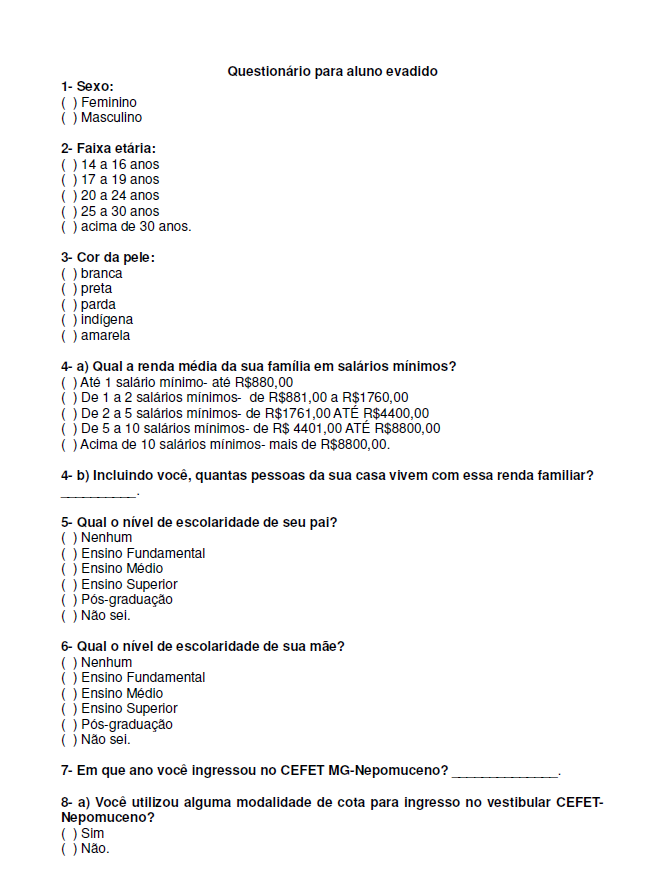
\includegraphics[width=16cm,cfbox=black 1pt 1pt]{graphics/fig-questionario.png}          % apendices (opcional)

% \addcontentsline{toc}{section}{\protect\numberline{}APÊNDICE B - XXXX XXXXX}
% \section*{\centering APÊNDICE B - XXXXXXX XXXXX}

\justifying
Apêndices são elementos pos textuais produzidos pelo autor da obra. Já anexos, são elementos pos textuais de terceiros.           % apendices (opcional)

% \addcontentsline{toc}{section}{\protect\numberline{}ANEXO A - LISTA DE ABREVIATURAS}
% \include{posTextual/anexoa}          % anexos (opcional)
% \addcontentsline{toc}{section}{\protect\numberline{}ANEXO B - ABREVIATURAS DE MESES}
% \include{posTextual/anexob}          % anexos (opcional)

\end{document}
